\newpage

\underline{\textbf{Answers to Tutorial Exercises - Chapter \thechapter}}

\begin{enumerate}
[   topsep  = 3ex
,   itemsep = 4ex
,   parsep  = 2ex
]
\item
    \begin{enumerate}
    [   topsep = 0ex
    ]
    \item
        \begin{minipage}[t]{0.49\linewidth}
            \vspace{-2em}
            \begin{align*}
                A = \begin{pmatrix}
                    1 & 1 & 0 & 0 & 1 & 0\\
                    1 & 1 & 1 & 0 & 0 & 1\\
                    0 & 1 & 1 & 0 & 0 & 0\\
                    0 & 0 & 0 & 1 & 1 & 0\\
                    1 & 0 & 0 & 1 & 1 & 1\\
                    0 & 1 & 0 & 0 & 1 & 1\\
                \end{pmatrix}
            \end{align*}
            \begin{lstlisting}
% Exercise 7-qn1(a)
A=[
    1 1 0 0 1 0
    1 1 1 0 0 1
    0 1 1 0 0 0
    0 0 0 1 1 0
    1 0 0 1 1 1
    0 1 0 0 1 1];
xy=[1 1;3 1;4 1;
    1 2;2 2;4 2];
gplot(A,xy,'k-*');
axis([0 5 0 3]);
text(1,0.9,'1');
text(3,0.9,'2');
text(4,0.9,'3');
text(1,2.1,'4');
text(2,2.1,'5');
text(4,2.1,'6');
%End
            \end{lstlisting}
        \end{minipage}
        \begin{minipage}[t]{0.5\linewidth}
            \begin{center}
\begin{tikzpicture}
    [   baseline = {(current bounding box.north)}
    ]
    \begin{axis}
        [   width = 0.9\linewidth
        ,   xmin = 0
        ,   xmax = 5
        ,   xtick = {0,1,2,3,4,5}
        ,   ymin = 0
        ,   ymax = 3
        ,   ytick = {0,1,2,3}
        ]
        \plot [black, mark = *, mark options = {solid}]
        coordinates {(2,2)(1,1)(4,1)};
        \plot [black, mark = *, mark options = {solid}]
        coordinates {(1,2)(4,2)(3,1)};
        \node[anchor = north] at (axis cs:1,1) {1};
        \node[anchor = north] at (axis cs:3,1) {2};
        \node[anchor = north] at (axis cs:4,1) {3};
        \node[anchor = south] at (axis cs:1,2) {4};
        \node[anchor = south] at (axis cs:2,2) {5};
        \node[anchor = south] at (axis cs:4,2) {6};
    \end{axis}
\end{tikzpicture}
\end{center}

        \end{minipage}
\newpage
    \item
        \begin{minipage}[t]{0.49\linewidth}
            \vspace{-2em}
            \begin{align*}
                A = \begin{pmatrix}
                    1 & 1 & 0 & 0 & 0 & 1\\
                    1 & 1 & 0 & 0 & 1 & 0\\
                    0 & 0 & 1 & 0 & 1 & 0\\
                    0 & 0 & 0 & 1 & 0 & 1\\
                    0 & 1 & 1 & 0 & 1 & 0\\
                    1 & 0 & 0 & 1 & 0 & 1\\
                \end{pmatrix}
            \end{align*}
            \begin{lstlisting}
% Exercise 7-qn1(b)
A=[
    1 1 0 0 0 1
    1 1 0 0 1 0
    0 0 1 0 1 0
    0 0 0 1 0 1
    0 1 1 0 1 0
    1 0 0 1 0 1];
xy=[2 1;3 1;4 1;
    1 1;3 2;2 2];
gplot(A,xy,'k-*');
axis([0 5 0 3]);
text(2,0.9,'1');
text(3,0.9,'2');
text(4,0.9,'3');
text(1,0.9,'4');
text(3,2.1,'5');
text(2,2.1,'6');
%End
            \end{lstlisting}
        \end{minipage}
        \begin{minipage}[t]{0.5\linewidth}
            \input{main/07/c7ans1b.tex}
        \end{minipage}
    \end{enumerate}


\item

    Consider the following adjacency graph:
    \begin{center}
        \includegraphics{main/07/ch7ex3.tikz}
    \end{center}
    First we write down the associated adjacency matrix - it is most efficient
    to create a script file in MATLAB and type all of your matrices within this
    file for multiple use.

    \begin{minipage}[t]{0.49\linewidth}
        \begin{lstlisting}
A=[
    1 1 1 1 0 1 0 1 0 1
    1 1 1 0 0 0 0 0 0 0
    1 1 1 0 0 0 0 0 0 0
    1 0 0 1 0 1 0 1 0 0
    0 0 0 0 1 1 0 1 1 1
    1 0 0 1 1 1 1 1 0 0
    0 0 0 0 0 1 1 0 0 0
    1 0 0 1 1 1 0 1 1 1
    0 0 0 0 1 0 0 1 1 1
    1 0 0 0 1 0 0 1 1 1]
        \end{lstlisting}
        In MATLAB use the command \textit{spy(A)} to find the pattern and the
        number of nonzero elements: i.e.\\
        \texttt{>> spy(A)}
    \end{minipage}
    \begin{minipage}[t]{0.5\linewidth}
        \input{main/07/c7ans2.tex}
    \end{minipage}

    You can find the hald bandwitch of $A$ using the following commands:
    \begin{lstlisting}
>> [i,j]=find(A);
>> bw=max(i-j)

bw =
    9
    \end{lstlisting}
    Therefore the full bandwidth is $= 9 + 9 + 1 = 19$

    Next we apply the Cuthill-McKee (CM) and reverse Cuthill-McKee (RCM)
    ordering algorithms to reduce the bandwidth.

    we need to construct the following table
    \begin{center}
        \renewcommand{\arraystretch}{1.2}
        \setlength{\tabcolsep}{6pt}
        \begin{tabular}{p{15mm}p{20mm}p{15mm}p{18mm}p{16mm}p{16mm}p{15mm}}
            Original nodes & No. of connections & Results / Heads & Queue
            & Result by CM & Result by RCM & New nodes\\
            \hline
             1 & 6 &  7 & 6\\
             2 & 2 &  6 & 4, 5, 8, 1\\
             3 & 2 &  4 & --\\
             4 & 3 &  5 & 9, 10\\
             5 & 4 &  8 & --\\
             6 & 5 &  1 & 2, 3\\
             7 & 1 &  9 & --\\
             8 & 6 & 10 & --\\
             9 & 3 &  2 & --\\
            10 & 4 &  3 & --\\
        \end{tabular}
    \end{center}
    Step 1 - list all the nodes and the number of their connections (or degree)
    -- check this with the adjacency matrix as well.

    Step 2 - choose the node with smallest number of connections --  here is
    node 7 -- write it down under the Results/Heads column.
    Since node 7 is only connected to node 6 we write down 6 Queue column.
    Bring down 6 to the results column,

    Step 3 - next, in the Queue column write down the list of nodes which are
    connected to 6 (in the ascending order of their degree or number of
    connections).
    Bring 4 down and repeat Stage 3.
    Avoid writing the numbers which are already listed in the Queue column and
    the starting node 7 -- since 6, 1, and 8 are already in the Queue we put a
    -- for node 4 in the Queue column.

    Step 4 - we bring the next number down in the queue -- that is 5, and repeat
    stage 3.
    We only list 9 and 10, since 6 and 8 are already listed in the queue.

    Repeat Step 4 -- all the connections to node 8 already in the list, so we
    put a -- for node 8 in the Queue column.

    We bring 1 down which is connected to two new nodes 2 and 3, we write down
    2, 3 in the Queue column.

    Next, we bring 9 and follow the above procedure until all 10 nodes are
    listed in the results/Head column.

    \begin{center}
        \renewcommand{\arraystretch}{1.2}
        \setlength{\tabcolsep}{6pt}
        \begin{tabular}{p{15mm}p{20mm}p{15mm}p{18mm}p{16mm}p{16mm}p{15mm}}
            Original nodes & No. of connections & Results / Heads & Queue
            & Result by CM & Result by RCM & New nodes\\
            \hline
             1 & 6 &  7 & 6 &  7 & \tikzmark{B}3\tikzmark{C} & \tikzmark{D}1\\
             2 & 2 &  6 & 4, 5, 8, 1 &  6 &  2 &  2\\
             3 & 2 &  4 & --         &  4 & 10 &  3\\
             4 & 3 &  5 & 9, 10      &  5 &  9 &  4\\
             5 & 4 &  8 & --         &  8 &  1 &  5\\
             6 & 5 &  1 & 2, 3       &  1 &  8 &  6\\
             7 & 1 &  9 & --         &  9 &  5 &  7\\
             8 & 6 & 10 & --         & 10 &  4 &  8\\
             9 & 3 &  2 & --         &  2 &  6 &  9\\
            10 & 4 &  3 & -- &  3\tikzmark{A} &  7 & 10\\
        \end{tabular}
        \begin{tikzpicture}
            [   remember picture
            ,   overlay
            ,   > = Stealth
            ]
            \draw[<->] ($(pic cs:A)+(4pt,6pt)$) to[out=45, in=-135] ($(pic cs:B)+(-4pt,2pt)$);
            \draw[->] ($(pic cs:C)+(4pt,4pt)$) to ($(pic cs:D)+(-4pt,4pt)$);
        \end{tikzpicture}
    \end{center}

    Complete results column for CM (the same as the column Results / Heads) and
    then reverse the CM column for RCM method, and enter the column header
    `New nodes'.

    We now copy the original adjacency graph and go along the RCM column, and
    say that, the original node 3 becomes node 1, original node 2 remains node 2,
    original node 10 becomes 3, and so on.

    Repeat this for CM method.

    \begin{center}
        \includegraphics[width=0.45\linewidth]{main/07/ch7ex3orig.tikz}

        \vspace{1em}
        \includegraphics[width=0.45\linewidth]{main/07/ch7ex3cm.tikz}
        \hspace{\fill}
        \includegraphics[width=0.45\linewidth]{main/07/ch7ex3rcm.tikz}
    \end{center}

    \newpage
    Now use MATLAB to construct the adjacency matrix B and C associated with the
    reordered RCM adjacency plot:

    \begin{minipage}[t]{0.49\linewidth}
        \vspace{-2em}
        \begin{lstlisting}
B=[
    1 1 0 0 0 0 0 0 0 0
    1 1 1 1 1 1 0 0 0 0
    0 1 1 0 1 1 0 0 0 0
    0 1 0 1 1 0 1 1 0 0
    0 1 1 1 1 1 1 1 0 0
    0 1 1 0 1 1 0 1 1 1
    0 0 0 1 1 0 1 1 0 0
    0 0 0 1 1 1 1 1 0 0
    0 0 0 0 0 1 0 0 1 1
    0 0 0 0 0 1 0 0 1 1];
        \end{lstlisting}

        We can now find the bandwidth for the reordered matrix:
        \begin{lstlisting}
>> [i,j]=find(B);
>> bw=max(i-j)

bw = 4
        \end{lstlisting}
    \end{minipage}
    \begin{minipage}[t]{0.5\linewidth}
        \input{main/07/c7ans2B.tex}
    \end{minipage}

    Hence, the full bandwidth for the reordered matrix by CM method is
    $= 4 + 4 + 1 = 9$.

    \begin{minipage}[t]{0.49\linewidth}
        \begin{lstlisting}
C=[
    1 1 0 0 1 0 0 0 0 0
    1 1 0 0 1 0 0 0 0 0
    0 0 1 1 1 1 1 0 0 0
    0 0 1 1 0 1 1 0 0 0
    1 1 1 0 1 1 0 1 1 0
    0 0 1 1 1 1 1 1 1 0
    0 0 1 1 0 1 1 0 1 0
    0 0 0 0 1 1 0 1 1 0
    0 0 0 0 1 1 1 1 1 1
    0 0 0 0 0 0 0 0 1 1];
        \end{lstlisting}

        \begin{lstlisting}
>> [i,j]=find(B);
>> bw=max(i-j)

bw = 4
        \end{lstlisting}
    \end{minipage}
    \begin{minipage}[t]{0.5\linewidth}
        \input{main/07/c7ans2C.tex}
    \end{minipage}

    Hence, the full bandwidth for the reordered matrix by CM method is
    $= 4 + 4 + 1 = 9$.

    For this example matrix, both CM and RCM work equally well in reducing the
    bandwidth of the original matrix from 19 to 9.

    \newpage
    Next we use the MATLAB command \texttt{symrcm(A)} to test our RCM reordering
    result.

    \begin{minipage}[t]{0.49\linewidth}
        \begin{lstlisting}
>> p=symrcm(A);
>> spy(A(p,p))
        \end{lstlisting}

        Next we can find the corresponding bandwidth:

        \begin{lstlisting}
>> [i,j]=find(A(p,p));
>> bw=max(i-j)

bw = 4
        \end{lstlisting}

        Hence, the \texttt{symrcm} command also results in a full bandwidth of
        $= 4 + 4 + 1 = 9$.
    \end{minipage}
    \begin{minipage}[t]{0.5\linewidth}
        \begin{center}
\scriptsize
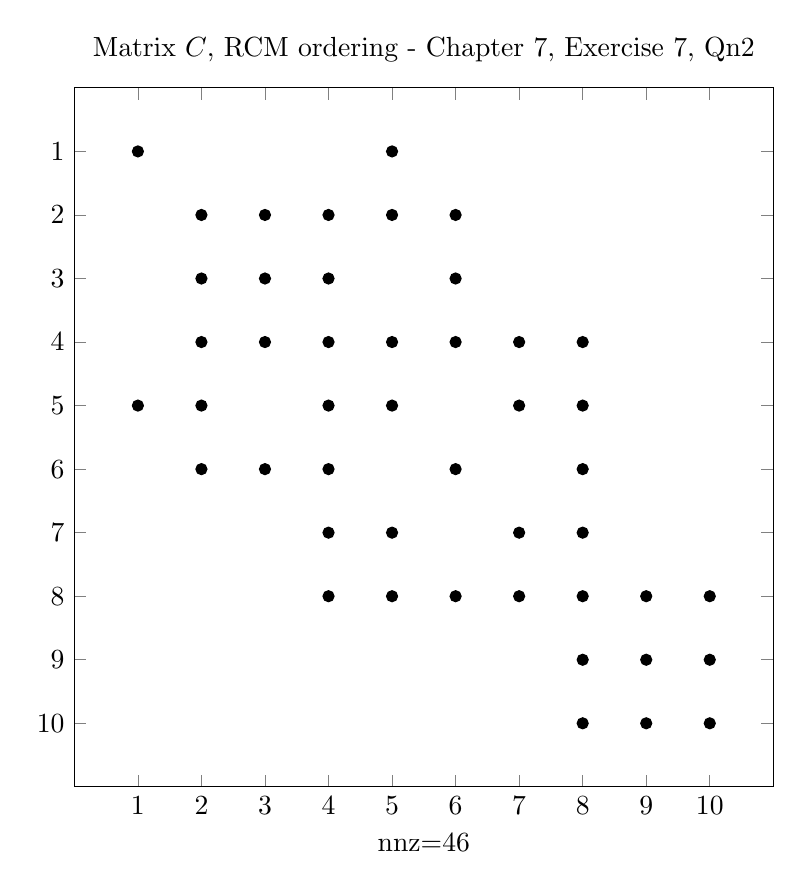
\begin{tikzpicture}
    [   baseline = {(current bounding box.north)}
    ]
    \begin{axis}
        [   unit vector ratio* = 1 1 1
        ,   y dir = reverse
        ,   xmin = 0
        ,   ymin = 0
        ,   xmax = 11
        ,   ymax = 11
        ,   title = {Matrix $C$, RCM ordering - Chapter 7, Exercise 7, Qn2}
        ,   xlabel = {nnz=46}
        ,   width = \linewidth
        ,   xtick = {1,2,3,4,5,6,7,8,9,10}
        ,   ytick = {1,2,3,4,5,6,7,8,9,10}
        ]
        \addplot[only marks] coordinates
        {   (1,1)               (5,1)
                 (2,2)(3,2)(4,2)(5,2)(6,2)
                 (2,3)(3,3)(4,3)     (6,3)
                 (2,4)(3,4)(4,4)(5,4)(6,4)(7,4)(8,4)
            (1,5)(2,5)     (4,5)(5,5)     (7,5)(8,5)
                 (2,6)(3,6)(4,6)     (6,6)     (8,6)
                           (4,7)(5,7)     (7,7)(8,7)
                           (4,8)(5,8)(6,8)(7,8)(8,8)(9,8)(10,8)
                                               (8,9)(9,9)(10,9)
                                              (8,10)(9,10)(10,10)
        };
    \end{axis}
\end{tikzpicture}
\end{center}

    \end{minipage}

    Reading form the plot of \texttt{symrcm} adjacency matrix, we can also write
    down the associated adjacency matrix and plot:

    \begin{minipage}[t]{0.49\linewidth}
        \begin{lstlisting}
A(p,p)=[
    1 0 0 0 1 0 0 0 0 0
    0 1 1 1 1 1 0 0 0 0
    0 1 1 1 0 1 0 0 0 0
    0 1 1 1 1 1 1 1 0 0
    1 1 0 1 1 0 1 1 0 0
    0 1 1 1 0 1 0 1 0 0
    0 0 0 1 1 1 1 1 1 1
    0 0 0 0 0 0 0 1 1 1
    0 0 0 0 0 0 0 1 1 1]
        \end{lstlisting}
    \end{minipage}
    \begin{minipage}[t]{0.5\linewidth}
        ~\\
        \includegraphics[width=0.9\linewidth]{main/07/ch7ex3sym.tikz}
    \end{minipage}

    \newpage
    \textbf{Column Count reordering:}

    \begin{center}
        \renewcommand{\arraystretch}{1.2}
        \setlength{\tabcolsep}{6pt}
        \begin{tabular}{r|>{\hspace*{\tabcolsep}}CCCCCCCCCC}
            vertex & 1 & 2 & 3 & 4 & 5 & 6 & 7 & 8 & 9 & 10\\
            \hline
            degree & 6 & 2 & 2 & 3 & 4 & 5 & 1 & 6 & 3 & 4\\
        \end{tabular}

        \begin{tabular}{r|>{\hspace*{\tabcolsep}}CCCCCCCCCC}
            vertex   & 1 & 2 & 3 & 4 & 5 & 6 & 7 & 8 & 9 & 10\\
            \hline
            original & 7\uparrow & 2\uparrow & 3\uparrow & 4\uparrow & 9\uparrow & 5\uparrow &10\uparrow & 6\uparrow & 1\uparrow & 8\uparrow\\
        \end{tabular}
    \end{center}
    \vspace{2em}
    \begin{center}
        \renewcommand{\arraystretch}{1.2}
        \setlength{\tabcolsep}{2ex}
        \begin{tabular}{p{0.45\linewidth}|p{0.45\linewidth}}
            \centering\includegraphics[width=0.9\linewidth]{main/07/ch7ex3orig.tikz} &
            \centering\includegraphics[width=0.9\linewidth]{main/07/ch7ex3cc.tikz}
            \arraybackslash\\
            ~\vspace{2em}

            $\scriptsize D = \begin{pmatrix}
                1 & 0 & 0 & 0 & 0 & 0 & 0 & 1 & 0 & 0\\
                0 & 1 & 1 & 0 & 0 & 0 & 0 & 0 & 1 & 0\\
                0 & 1 & 1 & 0 & 0 & 0 & 0 & 0 & 1 & 0\\
                0 & 0 & 0 & 1 & 0 & 0 & 0 & 1 & 1 & 1\\
                0 & 0 & 0 & 0 & 1 & 1 & 1 & 0 & 0 & 1\\
                0 & 0 & 0 & 0 & 1 & 1 & 1 & 1 & 0 & 1\\
                0 & 0 & 0 & 0 & 1 & 1 & 1 & 0 & 1 & 1\\
                1 & 0 & 0 & 1 & 0 & 1 & 0 & 1 & 1 & 1\\
                0 & 1 & 1 & 1 & 0 & 0 & 1 & 1 & 1 & 1\\
                0 & 0 & 0 & 1 & 1 & 1 & 1 & 1 & 1 & 1
            \end{pmatrix}$ &
            \begin{center}
\scriptsize
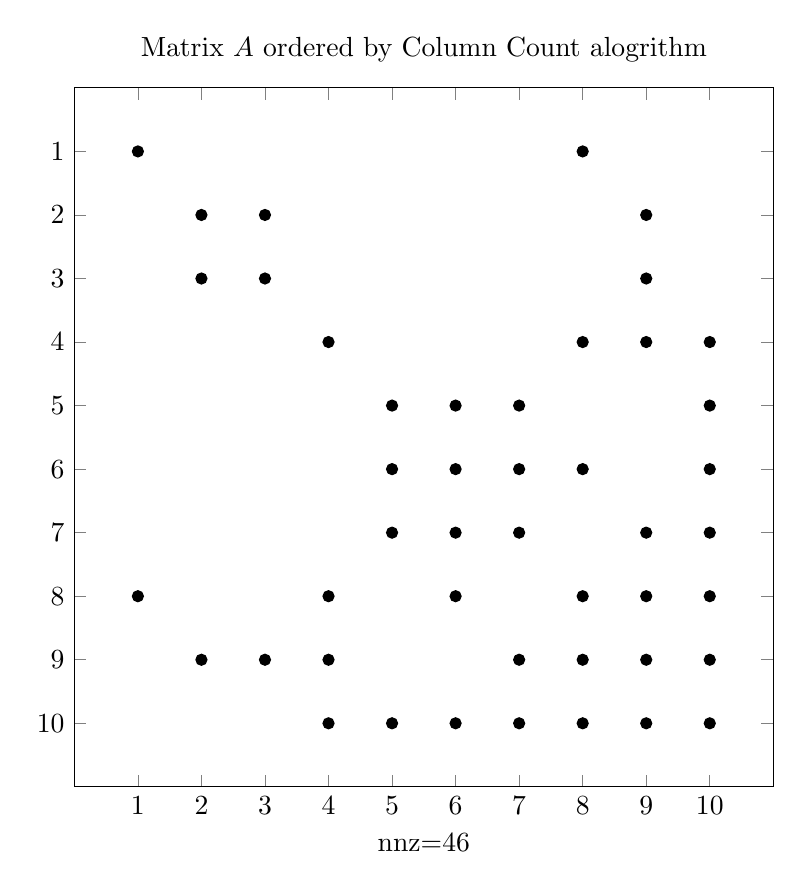
\begin{tikzpicture}
    [   baseline = {(current bounding box.north)}
    ]
    \begin{axis}
        [   unit vector ratio* = 1 1 1
        ,   y dir = reverse
        ,   xmin = 0
        ,   ymin = 0
        ,   xmax = 11
        ,   ymax = 11
        ,   title = {Matrix $A$ ordered by Column Count alogrithm}
        ,   xlabel = {nnz=46}
        ,   width = \linewidth
        ,   xtick = {1,2,3,4,5,6,7,8,9,10}
        ,   ytick = {1,2,3,4,5,6,7,8,9,10}
        ]
        \addplot[only marks] coordinates
        {   (1,1)                              (8,1)
                 (2,2)(3,2)                         (9,2)
                 (2,3)(3,3)                         (9,3)
                           (4,4)               (8,4)(9,4)(10,4)
                                (5,5)(6,5)(7,5)          (10,5)
                                (5,6)(6,6)(7,6)(8,6)     (10,6)
                                (5,7)(6,7)(7,7)     (9,7)(10,7)
            (1,8)          (4,8)     (6,8)     (8,8)(9,8)(10,8)
                 (2,9)(3,9)(4,9)          (7,9)(8,9)(9,9)(10,9)
                    (4,10)(5,10)(6,10)(7,10)(8,10)(9,10)(10,10)
        };
    \end{axis}
\end{tikzpicture}
\end{center}

            \\
            ~\vspace{2em}

            Note that D (ordered Matrix $A$ by Column Count algorithm) is identical to Matrix A ordered by using the MATLAB command \texttt{colperm} i.e.

            \begin{lstlisting}
>> q=colperm(A);
>> spy(A(q,q))
            \end{lstlisting}&
            \input{main/07/c7ans2colp.tex}
        \end{tabular}
    \end{center}

    \newpage
    \textbf{Minimum Degree reordering}

    \begin{center}
        \renewcommand{\arraystretch}{1}
        \setlength{\tabcolsep}{8pt}
        \begin{tabular}{rr|cccccccccc}
            \multicolumn{2}{l|}{New} & \multicolumn{10}{c}{vertex and number of degree}\\
            \multicolumn{2}{l|}{ordering} & 1 & 2 & 3 & 4 & 5 & 6 & 7 & 8 & 9 & 10\\
            \multicolumn{2}{C|}{\leftarrow} & 6 & 2 & 2 & 3 & 4 & 5 & 1 & 6 & 3 & 4\\
            \hline
            1 & 7 & 6 & 2 & 2 & 3 & 4 & 4 & X & 6 & 3 & 4\\
            2 & 2 & 5 & X & 1 & 3 & 4 & 4 & X & 6 & 3 & 4\\
            3 & 3 & 4 & X & X & 3 & 4 & 4 & X & 5 & 3 & 4\\
            4 & 4 & 3 & X & X & X & 4 & 3 & X & 5 & 3 & 4\\
            5 & 1 & X & X & X & X & 4 & 2 & X & 4 & 3 & 3\\
            6 & 6 & X & X & X & X & 3 & X & X & 3 & 3 & 3\\
            7 & 8 & X & X & X & X & 2 & X & X & X & 2 & 2\\
            8 & 5 & X & X & X & X & X & X & X & X & 1 & 1\\
            9 & 9 & X & X & X & X & X & X & X & X & X & 1\\
            10&10 & X & X & X & X & X & X & X & X & X & X\\
        \end{tabular}
    \end{center}
    \begin{center}
        \renewcommand{\arraystretch}{1}
        \setlength{\tabcolsep}{6pt}
        \begin{tabular}{p{0.45\linewidth}|p{0.45\linewidth}}
            ~\vspace{2em}

            $\scriptsize M = \begin{pmatrix}
                1 & 0 & 0 & 0 & 0 & 1 & 0 & 0 & 0 & 0\\
                0 & 1 & 1 & 0 & 1 & 0 & 0 & 0 & 0 & 0\\
                0 & 1 & 1 & 0 & 1 & 0 & 0 & 0 & 0 & 0\\
                0 & 0 & 0 & 1 & 1 & 1 & 1 & 0 & 0 & 0\\
                0 & 1 & 1 & 1 & 1 & 1 & 1 & 0 & 0 & 1\\
                1 & 0 & 0 & 1 & 1 & 1 & 1 & 1 & 0 & 0\\
                0 & 0 & 0 & 1 & 1 & 1 & 1 & 1 & 1 & 1\\
                0 & 0 & 0 & 0 & 0 & 0 & 1 & 1 & 1 & 1\\
                0 & 0 & 0 & 0 & 1 & 0 & 1 & 1 & 1 & 1
            \end{pmatrix}$ &
            ~\vspace{-2em}

            \centering\includegraphics[width=0.9\linewidth]{main/07/ch7ex3md.tikz}
            \arraybackslash\\
            \input{main/07/c7ans2syma.tex} &
            \input{main/07/c7ans2md.tex}\\
        \end{tabular}
    \end{center}

    \textbf{Comment} -- for this matrix, the MD algorithm seems to produce a
    reordered matrix very similar to the \texttt{sysamd} function within MATLAB,
    hence the algorithm works well.

    \textbf{Next we perform LU factorisation and check the number of nonzeros
    generated in the decomposition process}.

    See Figure 7.Q2, below. Compare the upper triangular matrix $U$ in each case
    with the corresponding full matrices, i.e. original matrix $A$, RCM ($C$),
    Column Count ($D$) and Minimum Degree ($M$), and write down the number of
    nonzeros generated for each case.
    The answer will be checked in the tutorial session.

    \begin{center}
        \renewcommand{\arraystretch}{0.6}
        \setlength{\tabcolsep}{6pt}
        \begin{tabular}{p{0.45\linewidth} p{0.45\linewidth}}
            \begin{center}
\scriptsize
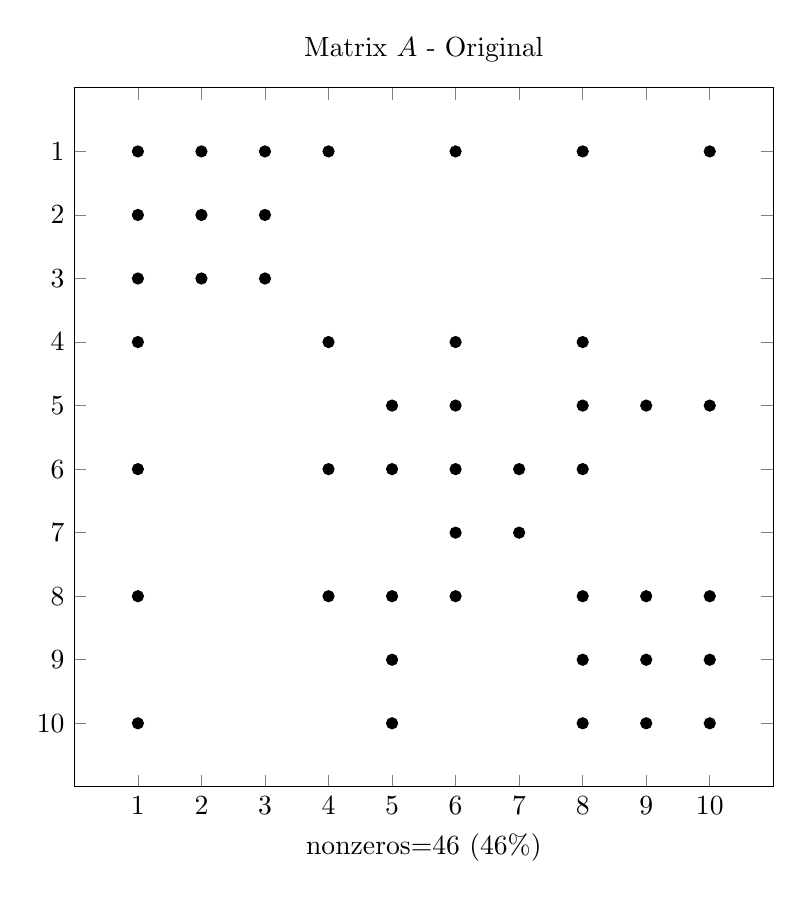
\begin{tikzpicture}
    [   baseline = {(current bounding box.north)}
    ]
    \begin{axis}
        [   unit vector ratio* = 1 1 1
        ,   y dir = reverse
        ,   xmin = 0
        ,   ymin = 0
        ,   xmax = 11
        ,   ymax = 11
        ,   title = {Matrix $A$ - Original}
        ,   xlabel = {nonzeros=46 (46\%)}
        ,   width = \linewidth
        ,   xtick = {1,2,3,4,5,6,7,8,9,10}
        ,   ytick = {1,2,3,4,5,6,7,8,9,10}
        ]
        \addplot[only marks] coordinates
        {   (1,1)(2,1)(3,1)(4,1)     (6,1)     (8,1)     (10,1)
            (1,2)(2,2)(3,2)
            (1,3)(2,3)(3,3)
            (1,4)          (4,4)     (6,4)     (8,4)
                                (5,5)(6,5)     (8,5)(9,5)(10,5)
            (1,6)          (4,6)(5,6)(6,6)(7,6)(8,6)
                                     (6,7)(7,7)
            (1,8)          (4,8)(5,8)(6,8)     (8,8)(9,8)(10,8)
                                (5,9)          (8,9)(9,9)(10,9)
            (1,10)              (5,10)      (8,10)(9,10)(10,10)
        };
    \end{axis}
\end{tikzpicture}
\end{center}
 & \begin{center}
\scriptsize
\begin{tikzpicture}
    [   baseline = {(current bounding box.north)}
    ]
    \begin{axis}
        [   unit vector ratio* = 1 1 1
        ,   y dir = reverse
        ,   xmin = 0
        ,   ymin = 0
        ,   xmax = 11
        ,   ymax = 11
        ,   title = {$[L,U]$ of Matrix $A$, $U$}
        ,   xlabel = {nonzeros=38 (38\%)}
        ,   width = \linewidth
        ,   xtick = {1,2,3,4,5,6,7,8,9,10}
        ,   ytick = {1,2,3,4,5,6,7,8,9,10}
        ]
        \addplot[only marks] coordinates
        {   (1,1)(2,1)(3,1)(4,1)     (6,1)     (8,1)     (10,1)
                 (2,2)(3,2)                              (10,2)
                           (4,3)     (6,3)     (8,3)     (10,3)
                           (4,4)     (6,4)     (8,4)     (10,4)
                                (5,5)(6,5)     (8,5)(9,5)(10,5)
                                     (6,6)(7,6)(8,6)(9,6)(10,6)
                                          (7,7)(8,7)(9,7)(10,7)
                                               (8,8)(9,8)(10,8)
                                                    (9,9)(10,9)
                                                         (10,10)
        };
    \end{axis}
\end{tikzpicture}
\end{center}
\\
            \begin{center}
\scriptsize
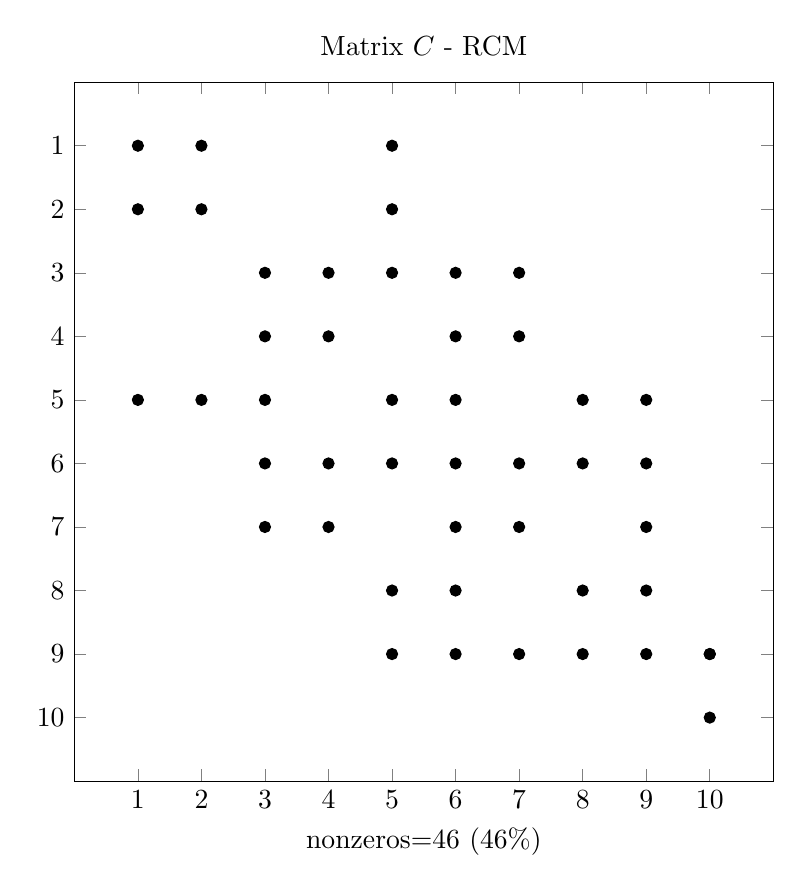
\begin{tikzpicture}
    [   baseline = {(current bounding box.north)}
    ]
    \begin{axis}
        [   unit vector ratio* = 1 1 1
        ,   y dir = reverse
        ,   xmin = 0
        ,   ymin = 0
        ,   xmax = 11
        ,   ymax = 11
        ,   title = {Matrix $C$ - RCM}
        ,   xlabel = {nonzeros=46 (46\%)}
        ,   width = \linewidth
        ,   xtick = {1,2,3,4,5,6,7,8,9,10}
        ,   ytick = {1,2,3,4,5,6,7,8,9,10}
        ]
        \addplot[only marks] coordinates
        {   (1,1)(2,1)          (5,1)
            (1,2)(2,2)          (5,2)
                      (3,3)(4,3)(5,3)(6,3)(7,3)
                      (3,4)(4,4)     (6,4)(7,4)
            (1,5)(2,5)(3,5)     (5,5)(6,5)     (8,5)(9,5)
                      (3,6)(4,6)(5,6)(6,6)(7,6)(8,6)(9,6)
                      (3,7)(4,7)     (6,7)(7,7)     (9,7)
                                (5,8)(6,8)     (8,8)(9,8)
                                (5,9)(6,9)(7,9)(8,9)(9,9)(10,9)
                                                   (10,9)(10,10)
        };
    \end{axis}
\end{tikzpicture}
\end{center}
 & \begin{center}
\scriptsize
\begin{tikzpicture}
    [   baseline = {(current bounding box.north)}
    ]
    \begin{axis}
        [   unit vector ratio* = 1 1 1
        ,   y dir = reverse
        ,   xmin = 0
        ,   ymin = 0
        ,   xmax = 11
        ,   ymax = 11
        ,   title = {$[L,U]$ Matrix $C$, $U$}
        ,   xlabel = {nonzeros=23 (23\%)}
        ,   width = \linewidth
        ,   xtick = {1,2,3,4,5,6,7,8,9,10}
        ,   ytick = {1,2,3,4,5,6,7,8,9,10}
        ]
        \addplot[only marks] coordinates
        {   (1,1)(2,1)          (5,1)

                      (3,3)(4,3)(5,3)(6,3)(7,3)
                           (4,4)(5,4)     (7,4)(8,4)(9,4)
                                (5,5)
                                     (6,6)     (8,6)(9,6)
                                          (7,7)          (10,7)
                                               (8,8)(9,8)
                                                    (9,9)
                                                         (10,10)
        };
    \end{axis}
\end{tikzpicture}
\end{center}
\\
            \input{main/07/c7ans2fD.tex} & \begin{center}
\scriptsize
\begin{tikzpicture}
    [   baseline = {(current bounding box.north)}
    ]
    \begin{axis}
        [   unit vector ratio* = 1 1 1
        ,   y dir = reverse
        ,   xmin = 0
        ,   ymin = 0
        ,   xmax = 11
        ,   ymax = 11
        ,   title = {$[L,U]$ of Matrix $D$, $U$}
        ,   xlabel = {nonzeros=20 (20\%)}
        ,   width = \linewidth
        ,   xtick = {1,2,3,4,5,6,7,8,9,10}
        ,   ytick = {1,2,3,4,5,6,7,8,9,10}
        ]
        \addplot[only marks] coordinates
        {   (1,1)                              (8,1)
                 (2,2)(3,2)                         (9,2)

                           (4,4)               (8,4)(9,4)(10,4)
                                (5,5)(6,5)(7,5)          (10,5)
                                     (6,6)     (8,6)
                                          (7,7)     (9,7)
                                               (8,8)
                                                    (9,9)
                                                         (10,10)
        };
    \end{axis}
\end{tikzpicture}
\end{center}
\\
            \begin{center}
\scriptsize
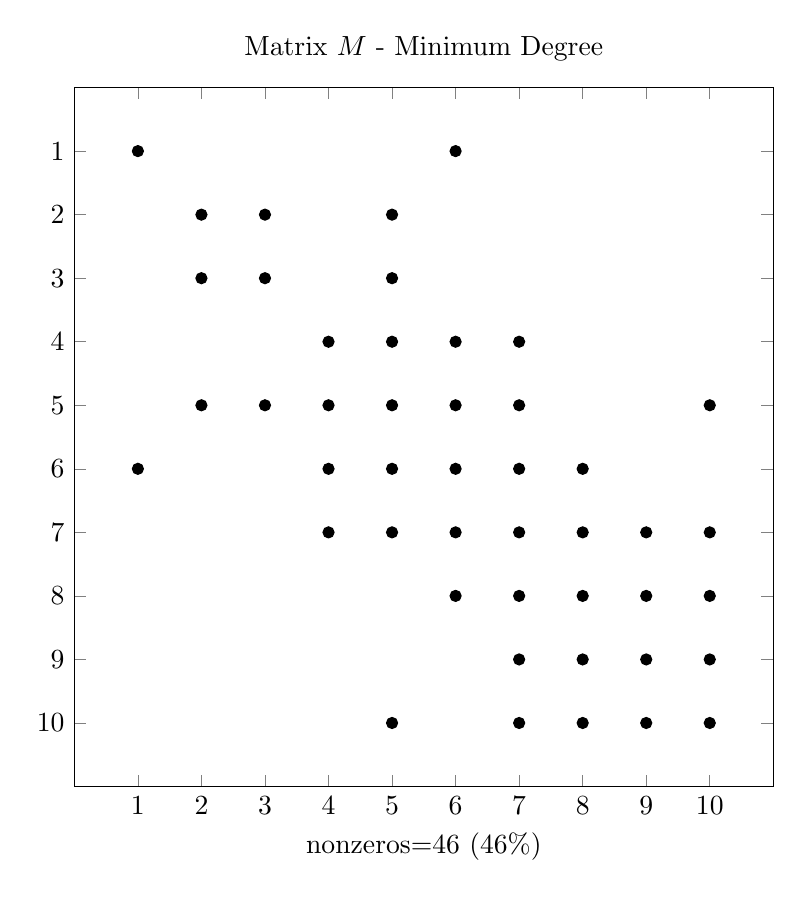
\begin{tikzpicture}
    [   baseline = {(current bounding box.north)}
    ]
    \begin{axis}
        [   unit vector ratio* = 1 1 1
        ,   y dir = reverse
        ,   xmin = 0
        ,   ymin = 0
        ,   xmax = 11
        ,   ymax = 11
        ,   title = {Matrix $M$ - Minimum Degree}
        ,   xlabel = {nonzeros=46 (46\%)}
        ,   width = \linewidth
        ,   xtick = {1,2,3,4,5,6,7,8,9,10}
        ,   ytick = {1,2,3,4,5,6,7,8,9,10}
        ]
        \addplot[only marks] coordinates
        {   (1,1)                    (6,1)
                 (2,2)(3,2)     (5,2)
                 (2,3)(3,3)     (5,3)
                           (4,4)(5,4)(6,4)(7,4)
                 (2,5)(3,5)(4,5)(5,5)(6,5)(7,5)          (10,5)
            (1,6)          (4,6)(5,6)(6,6)(7,6)(8,6)
                           (4,7)(5,7)(6,7)(7,7)(8,7)(9,7)(10,7)
                                     (6,8)(7,8)(8,8)(9,8)(10,8)
                                          (7,9)(8,9)(9,9)(10,9)
                                (5,10)  (7,10)(8,10)(9,10)(10,10)
        };
    \end{axis}
\end{tikzpicture}
\end{center}
 & \input{main/07/c7ans2fMU.tex}\\
        \end{tabular}
    \end{center}
    Figure 7.Q2 Comparison of ordering schemes (using the algorithms shown in
    \break Chapter 7), and their $LU$ factorisation showing fill-ins reduction.

    \newpage
    \begin{minipage}[t]{0.5\linewidth}
        \begin{align*}
            \scriptsize
            A = \begin{pmatrix}
                1 & 0 & 1 & 0 & 0 & 0 & 0 & 1 & 1\\
                0 & 1 & 1 & 0 & 0 & 0 & 1 & 1 & 0\\
                1 & 1 & 1 & 0 & 0 & 0 & 0 & 0 & 0\\
                0 & 0 & 0 & 1 & 0 & 0 & 0 & 1 & 1\\
                0 & 0 & 0 & 0 & 1 & 0 & 1 & 1 & 0\\
                0 & 0 & 0 & 0 & 0 & 1 & 1 & 0 & 0\\
                0 & 1 & 0 & 0 & 1 & 1 & 1 & 0 & 0\\
                1 & 1 & 0 & 1 & 1 & 0 & 0 & 1 & 0\\
                1 & 0 & 0 & 1 & 0 & 0 & 0 & 0 & 1
            \end{pmatrix}
        \end{align*}
    \end{minipage}
    \begin{minipage}[t]{0.45\linewidth}
        \begin{center}
\begin{tikzpicture}
    [   baseline = {(current bounding box.north)}
    ]
    \begin{axis}
        [   width = \linewidth
        ,   xmin = 0.5
        ,   xmax = 4.5
        ,   xtick = \empty
        ,   ymin = 0.5
        ,   ymax = 3.5
        ,   ytick = \empty
        ,   hide axis
        ]
        \plot [black, mark = *, mark options = {solid}]
        coordinates {(2,1)(2,2)(2,3)(4,3)};
        \plot [black, mark = *, mark options = {solid}]
        coordinates {(3,3)(3,1)(1,1)(1,2)(3,2)};
        \node[anchor = north east] at (axis cs:1,1) {9};
        \node[anchor = north east] at (axis cs:2,1) {1};
        \node[anchor = north west] at (axis cs:3,1) {3};
        \node[anchor = south east] at (axis cs:1,2) {4};
        \node[anchor = south east] at (axis cs:2,2) {8};
        \node[anchor = south west] at (axis cs:3,2) {2};
        \node[anchor = south east] at (axis cs:2,3) {5};
        \node[anchor = south west] at (axis cs:3,3) {7};
        \node[anchor = south west] at (axis cs:4,3) {6};
    \end{axis}
\end{tikzpicture}
\end{center}

    \end{minipage}

    \textbf{CM and RCM reordering:}
    \begin{center}
        \renewcommand{\arraystretch}{0.9}
        \setlength{\tabcolsep}{6pt}
        \begin{tabular}{lllllll}
            Original & No. of & Results / & Queue & Result & Result & New\\
            nodes    & conn   & Heads     &       & by CM  & by RCM & nodes\\
            \hline
            1 & 3 & 6 & 7   & 6 & 9 $\rightarrow$ & 1\rule[1pt]{0pt}{1em}\\
            2 & 3 & 7 & 5,2 & 7 & 1 $\rightarrow$ & 2\\
            3 & 2 & 5 & 8   & 5 & 4 $\rightarrow$ & 3\\
            4 & 2 & 2 & 3   & 2 & 3 $\rightarrow$ & 4\\
            5 & 2 & 8 & 4,1 & 8 & 8 $\rightarrow$ & 5\\
            6 & 1 & 3 & --  & 3 & 2 $\rightarrow$ & 6\\
            7 & 3 & 4 & 9   & 4 & 5 $\rightarrow$ & 7\\
            8 & 4 & 1 & --  & 1 & 7 $\rightarrow$ & 8\\
            9 & 2 & 9 & --  & 9 & 6 $\rightarrow$ & 9\\
        \end{tabular}
    \end{center}
    \begin{minipage}[t]{0.5\linewidth}
        \begin{align*}
            \scriptsize
            B = \begin{pmatrix}
                1 & 1 & 0 & 0 & 0 & 0 & 0 & 0 & 0\\
                1 & 1 & 1 & 1 & 0 & 0 & 0 & 0 & 0\\
                0 & 1 & 1 & 0 & 1 & 0 & 0 & 0 & 0\\
                0 & 1 & 0 & 1 & 1 & 1 & 0 & 0 & 0\\
                0 & 0 & 1 & 1 & 1 & 0 & 1 & 1 & 0\\
                0 & 0 & 0 & 1 & 0 & 1 & 0 & 1 & 0\\
                0 & 0 & 0 & 0 & 1 & 0 & 1 & 0 & 1\\
                0 & 0 & 0 & 0 & 1 & 1 & 0 & 1 & 1\\
                0 & 0 & 0 & 0 & 0 & 0 & 1 & 1 & 1
            \end{pmatrix}
        \end{align*}
    \end{minipage}
    \begin{minipage}[t]{0.45\linewidth}
        \input{main/07/c7ans3gB.tex}
    \end{minipage}
    \begin{minipage}[t]{0.5\linewidth}
        \begin{align*}
            \scriptsize
            C = \begin{pmatrix}
                1 & 1 & 1 & 0 & 0 & 0 & 0 & 0 & 0\\
                1 & 1 & 0 & 1 & 1 & 0 & 0 & 0 & 0\\
                1 & 0 & 1 & 0 & 1 & 0 & 0 & 0 & 0\\
                0 & 1 & 0 & 1 & 0 & 1 & 0 & 0 & 0\\
                0 & 1 & 1 & 0 & 1 & 1 & 1 & 0 & 0\\
                0 & 0 & 0 & 1 & 1 & 1 & 0 & 1 & 0\\
                0 & 0 & 0 & 0 & 1 & 0 & 1 & 1 & 0\\
                0 & 0 & 0 & 0 & 0 & 1 & 1 & 1 & 1\\
                0 & 0 & 0 & 0 & 0 & 0 & 0 & 1 & 1
            \end{pmatrix}
        \end{align*}
    \end{minipage}
    \begin{minipage}[t]{0.45\linewidth}
        \input{main/07/c7ans3gC.tex}
    \end{minipage}
    \begin{minipage}[t]{0.45\linewidth}
        \begin{lstlisting}
>> [i,j]=find(A);
>> bw=max(i-j), bw=8,
        \end{lstlisting}
        full bandwidth$= 8 \times 2 + 1 = 17$
        %\vspace{1em}
        \begin{lstlisting}
>> [i,j]=find(C);
>> bw=max(i-j), bw=3,
        \end{lstlisting}
        full bandwidth$= 3 \times 2 + 1 = 7$
    \end{minipage}\quad
    \begin{minipage}[t]{0.45\linewidth}
        \begin{lstlisting}
>> [i,j]=find(B);
>> bw=max(i-j), bw=3,
        \end{lstlisting}
        full bandwidth$= 3 \times 2 + 1 = 7$
        %\vspace{1em}
        \begin{lstlisting}
>> p=symrcm(A);
>> spy(A(p,p))
>> [i,j]=find(A(p,p));
>> bw=max(i-j), bw=3,
        \end{lstlisting}
        full bandwidth$= 3 \times 2 + 1 = 7$
    \end{minipage}

    \begin{center}
        \renewcommand{\arraystretch}{1}
        \setlength{\tabcolsep}{6pt}
        \begin{tabular}{p{0.45\linewidth} p{0.45\linewidth}}
            \begin{center}
\scriptsize
\begin{tikzpicture}
    [   baseline = {(current bounding box.north)}
    ]
    \begin{axis}
        [   unit vector ratio* = 1 1 1
        ,   y dir = reverse
        ,   xmin = 0
        ,   ymin = 0
        ,   xmax = 10
        ,   ymax = 10
        ,   title = {Original Matrix $A$}
        ,   xlabel = {nnz=31}
        ,   width = \linewidth
        ,   xtick = {1,3,5,7,9}
        ,   ytick = {1,3,5,7,9}
        ]
        \addplot[only marks] coordinates
        {   (1,1)(1,3)(1,8)(1,9)
            (2,2)(2,3)(2,7)(2,8)
            (3,1)(3,2)(3,3)
            (4,4)(4,8)(4,9)
            (5,5)(5,7)(5,8)
            (6,6)(6,7)
            (7,2)(7,5)(7,6)(7,7)
            (8,1)(8,2)(8,4)(8,5)(8,8)
            (9,1)(9,4)(9,9)
        };
    \end{axis}
\end{tikzpicture}
\end{center}
 & \begin{center}
\scriptsize
\begin{tikzpicture}
    [   baseline = {(current bounding box.north)}
    ]
    \begin{axis}
        [   unit vector ratio* = 1 1 1
        ,   y dir = reverse
        ,   xmin = 0
        ,   ymin = 0
        ,   xmax = 10
        ,   ymax = 10
        ,   title = {Matrix $B$ CM}
        ,   xlabel = {nnz=31}
        ,   width = \linewidth
        ,   xtick = {1,3,5,7,9}
        ,   ytick = {1,3,5,7,9}
        ]
        \addplot[only marks] coordinates
        {   (1,1)(1,2)
            (2,1)(2,2)(2,3)(2,4)
            (3,2)(3,3)(3,5)
            (4,2)(4,4)(4,5)(4,6)
            (5,3)(5,4)(5,5)(5,7)(5,8)
            (6,4)(6,6)(6,8)
            (7,5)(7,7)(7,9)
            (8,5)(8,6)(8,8)(8,9)
            (9,7)(9,8)(9,9)
        };
    \end{axis}
\end{tikzpicture}
\end{center}
\\
            \begin{center}
\scriptsize
\begin{tikzpicture}
    [   baseline = {(current bounding box.north)}
    ]
    \begin{axis}
        [   unit vector ratio* = 1 1 1
        ,   y dir = reverse
        ,   xmin = 0
        ,   ymin = 0
        ,   xmax = 10
        ,   ymax = 10
        ,   title = {Matrix $C$ RCM}
        ,   xlabel = {nnz=31}
        ,   width = \linewidth
        ,   xtick = {1,3,5,7,9}
        ,   ytick = {1,3,5,7,9}
        ]
        \addplot[only marks] coordinates
        {   (1,1)(1,2)(1,3)
            (2,1)(2,2)(2,4)(2,5)
            (3,1)(3,3)(3,5)
            (4,2)(4,4)(4,6)
            (5,2)(5,3)(5,5)(5,6)(5,7)
            (6,4)(6,5)(6,6)(6,8)
            (7,5)(7,7)(7,8)
            (8,6)(8,7)(8,8)(8,9)
            (9,8)(9,9)
        };
    \end{axis}
\end{tikzpicture}
\end{center}
 & \begin{center}
\scriptsize
\begin{tikzpicture}
    [   baseline = {(current bounding box.north)}
    ]
    \begin{axis}
        [   unit vector ratio* = 1 1 1
        ,   y dir = reverse
        ,   xmin = 0
        ,   ymin = 0
        ,   xmax = 10
        ,   ymax = 10
        ,   title = {Matrix $A(p,p)$ \texttt{symrcm}}
        ,   xlabel = {nnz=31}
        ,   width = \linewidth
        ,   xtick = {1,3,5,7,9}
        ,   ytick = {1,3,5,7,9}
        ]
        \addplot[only marks] coordinates
        {   (1,1)(1,2)
            (2,1)(2,2)(2,3)(2,4)
            (3,2)(3,3)(3,5)(3,6)
            (4,2)(4,4)(4,6)
            (5,3)(5,5)(5,7)
            (6,3)(6,4)(6,6)(6,7)(6,8)
            (7,5)(7,6)(7,7)(7,9)
            (8,6)(8,8)(8,9)
            (9,7)(9,8)(9,9)
        };
    \end{axis}
\end{tikzpicture}
\end{center}
\\
        \end{tabular}
    \end{center}

    \textbf{Column Count reordering:}

    \begin{center}
        \renewcommand{\arraystretch}{1.2}
        \setlength{\tabcolsep}{6pt}
        \begin{tabular}{r|>{\hspace*{\tabcolsep}}CCCCCCCCC}
            vertex & 1 & 2 & 3 & 4 & 5 & 6 & 7 & 8 & 9\\
            \hline
            degree & 3 & 3 & 2 & 2 & 2 & 1 & 3 & 4 & 2\\
        \end{tabular}

        \begin{tabular}{r|>{\hspace*{\tabcolsep}}CCCCCCCCC}
            vertex & 1 & 2 & 3 & 4 & 5 & 6 & 7 & 8 & 9\\
            \hline
            Original & 6\uparrow & 3\uparrow & 4\uparrow & 5\uparrow &
            9\uparrow & 1\uparrow & 2\uparrow & 7\uparrow & 8\uparrow\\
        \end{tabular}
    \end{center}
    \begin{minipage}[t]{0.45\linewidth}
        \scriptsize
        \begin{align*}
            D = \begin{pmatrix}
                1 & 0 & 0 & 0 & 0 & 0 & 0 & 1 & 0\\
                0 & 1 & 0 & 0 & 0 & 1 & 1 & 0 & 0\\
                0 & 0 & 1 & 0 & 1 & 0 & 0 & 0 & 1\\
                0 & 0 & 0 & 1 & 0 & 0 & 0 & 1 & 1\\
                0 & 0 & 1 & 0 & 1 & 1 & 0 & 0 & 0\\
                0 & 1 & 0 & 0 & 1 & 1 & 0 & 0 & 1\\
                0 & 1 & 0 & 0 & 0 & 0 & 1 & 1 & 1\\
                1 & 0 & 0 & 1 & 0 & 0 & 1 & 1 & 0\\
                0 & 0 & 1 & 1 & 0 & 1 & 1 & 0 & 1
            \end{pmatrix}
        \end{align*}
    \end{minipage}
    \begin{minipage}[t]{0.45\linewidth}
        \begin{center}
\begin{tikzpicture}
    [   baseline = {(current bounding box.north)}
    ]
    \begin{axis}
        [   width = \linewidth
        ,   xmin = 0.5
        ,   xmax = 4.5
        ,   xtick = \empty
        ,   ymin = 0.5
        ,   ymax = 3.5
        ,   ytick = \empty
        ,   hide axis
        ]
        \plot [black, mark = *, mark options = {solid}]
        coordinates {(2,1)(2,2)(2,3)(4,3)};
        \plot [black, mark = *, mark options = {solid}]
        coordinates {(3,3)(3,1)(1,1)(1,2)(3,2)};
        \node[anchor = north east] at (axis cs:1,1) {5};
        \node[anchor = north east] at (axis cs:2,1) {6};
        \node[anchor = north west] at (axis cs:3,1) {2};
        \node[anchor = south east] at (axis cs:1,2) {3};
        \node[anchor = south east] at (axis cs:2,2) {9};
        \node[anchor = south west] at (axis cs:3,2) {7};
        \node[anchor = south east] at (axis cs:2,3) {4};
        \node[anchor = south west] at (axis cs:3,3) {8};
        \node[anchor = south west] at (axis cs:4,3) {1};
    \end{axis}
\end{tikzpicture}
\end{center}

    \end{minipage}

    \newpage
    \begin{minipage}[t]{0.45\linewidth}
        \input{main/07/c7ans2pD.tex}
        %\texttt{>> spy(D),title('Matrix D CC')}
\begin{lstlisting}
>> spy(D),title('Matrix D CC')
\end{lstlisting}        
    \end{minipage}\hspace*{\fill}
    \begin{minipage}[t]{0.45\linewidth}
        \begin{center}
\scriptsize
\begin{tikzpicture}
    [   baseline = {(current bounding box.north)}
    ]
    \begin{axis}
        [   unit vector ratio* = 1 1 1
        ,   y dir = reverse
        ,   xmin = 0
        ,   ymin = 0
        ,   xmax = 10
        ,   ymax = 10
        ,   title = {Matrix $A(q,q)$ \texttt{colperm}}
        ,   xlabel = {nnz=31}
        ,   width = \linewidth
        ,   xtick = {1,3,5,7,9}
        ,   ytick = {1,3,5,7,9}
        ]
        \addplot[only marks] coordinates
        {   (1,1)(1,8)
            (2,2)(2,6)(2,7)
            (3,3)(3,5)(3,9)
            (4,4)(4,8)(4,9)
            (5,3)(5,5)(5,6)
            (6,2)(6,5)(6,6)(6,9)
            (7,2)(7,7)(7,8)(7,9)
            (8,1)(8,4)(8,7)(8,8)
            (9,3)(9,4)(9,6)(9,7)(9,9)
        };
    \end{axis}
\end{tikzpicture}
\end{center}

\begin{lstlisting}
>> q=colperm(A);
>> spy(A(q,q)),title('Matrix A(q,q) colperm')
\end{lstlisting}
        %\texttt{>> q=colperm(A);}\\
        %\texttt{>> spy(A(q,q)),title('Matrix A(q,q) colperm')}
    \end{minipage}\hspace*{\fill}

    \textbf{Comment} -- For this matrix, the MD algorithm works well and
    produces a reordered matrix exactly the same as the \texttt{colperm}
    function in MATLAB.

    \textbf{Minimum Degree reordering}
    \begin{center}
        \renewcommand{\arraystretch}{1}
        \setlength{\tabcolsep}{8pt}
        \begin{tabular}{rr|ccccccccc}
            \multicolumn{2}{l|}{New} & \multicolumn{9}{c}{vertex and number of degree}\\
            \multicolumn{2}{l|}{ordering} & 1 & 2 & 3 & 4 & 5 & 6 & 7 & 8 & 9\\
            \multicolumn{2}{C|}{\leftarrow} & 3 & 3 & 2 & 2 & 2 & 1 & 3 & 4 & 2\\
            \hline
            1 & 6 & 3 & 3 & 2 & 2 & 2 & X & 2 & 4 & 2\\
            2 & 3 & 2 & 2 & X & 2 & 2 & X & 2 & 4 & 2\\
            3 & 1 & X & 2 & X & 2 & 2 & X & 2 & 3 & 1\\
            4 & 9 & X & 2 & X & 1 & 2 & X & 2 & 3 & X\\
            5 & 4 & X & 2 & X & X & 2 & X & 2 & 2 & X\\
            6 & 7 & X & 2 & X & X & 2 & X & X & 2 & X\\
            7 & 2 & X & X & X & X & 1 & X & X & 1 & X\\
            8 & 5 & X & X & X & X & X & X & X & 1 & X\\
            9 & 8 & X & X & X & X & X & X & X & X & X\\
        \end{tabular}
    \end{center}
    \begin{minipage}[t]{0.45\linewidth}
        \begin{center}
\begin{tikzpicture}
    [   baseline = {(current bounding box.north)}
    ]
    \begin{axis}
        [   width = \linewidth
        ,   xmin = 0.5
        ,   xmax = 4.5
        ,   xtick = \empty
        ,   ymin = 0.5
        ,   ymax = 3.5
        ,   ytick = \empty
        ,   hide axis
        ]
        \plot [black, mark = *, mark options = {solid}]
        coordinates {(2,1)(2,2)(2,3)(4,3)};
        \plot [black, mark = *, mark options = {solid}]
        coordinates {(3,3)(3,1)(1,1)(1,2)(3,2)};
        \node[anchor = north east] at (axis cs:1,1) {9};
        \node[anchor = north east] at (axis cs:2,1) {1};
        \node[anchor = north west] at (axis cs:3,1) {3};
        \node[anchor = south east] at (axis cs:1,2) {4};
        \node[anchor = south east] at (axis cs:2,2) {8};
        \node[anchor = south west] at (axis cs:3,2) {2};
        \node[anchor = south east] at (axis cs:2,3) {5};
        \node[anchor = south west] at (axis cs:3,3) {7};
        \node[anchor = south west] at (axis cs:4,3) {6};
    \end{axis}
\end{tikzpicture}
\end{center}

        \begin{center}
\scriptsize
\begin{tikzpicture}
    [   baseline = {(current bounding box.north)}
    ]
    \begin{axis}
        [   unit vector ratio* = 1 1 1
        ,   y dir = reverse
        ,   xmin = 0
        ,   ymin = 0
        ,   xmax = 10
        ,   ymax = 10
        ,   title = {$A(r,r)$ - Minimum Degree by \texttt{symamd}}
        ,   xlabel = {nnz=31}
        ,   width = \linewidth
        ,   xtick = {1,3,5,7,9}
        ,   ytick = {1,3,5,7,9}
        ]
        \addplot[only marks] coordinates
        {   (1,1)(1,2)
            (2,1)(2,2)(2,3)(2,4)
            (3,2)(3,3)(3,6)
            (4,2)(4,4)(4,5)(4,6)
            (5,4)(5,5)(5,7)
            (6,3)(6,4)(6,6)(6,7)(6,9)
            (7,5)(7,6)(7,7)(7,8)
            (8,7)(8,8)(8,9)
            (9,6)(9,8)(9,9)
        };
    \end{axis}
\end{tikzpicture}
\end{center}

    \end{minipage}\hspace*{\fill}
    \begin{minipage}[t]{0.45\linewidth}
        \input{main/07/c7ans3gM.tex}
        \begin{center}
\scriptsize
\begin{tikzpicture}
    [   baseline = {(current bounding box.north)}
    ]
    \begin{axis}
        [   unit vector ratio* = 1 1 1
        ,   y dir = reverse
        ,   xmin = 0
        ,   ymin = 0
        ,   xmax = 10
        ,   ymax = 10
        ,   title = {Original Matrix $A$}
        ,   xlabel = {nnz=31}
        ,   width = \linewidth
        ,   xtick = {1,3,5,7,9}
        ,   ytick = {1,3,5,7,9}
        ]
        \addplot[only marks] coordinates
        {
            (1,1)(1,6)
            (2,2)(2,3)(2,7)
            (3,2)(3,3)(3,4)(3,9)
            (4,3)(4,4)(4,5)
            (5,4)(5,5)(5,9)
            (6,1)(6,6)(6,7)(6,8)
            (7,2)(7,6)(7,7)(7,9)
            (8,6)(8,8)(8,9)
            (9,3)(9,5)(9,7)(9,8)(9,9)
        };
    \end{axis}
\end{tikzpicture}
\end{center}

    \end{minipage}\hspace*{\fill}

    \textbf{Comment} -- the MD algorithm does not seem to work as well as the
    \texttt{sysamd} function MATLAB.

    \textbf{Storage consideration}

    The following MATLAB commands provide information on sparse and full
    matrices storage organisation.
    \begin{lstlisting}
>> S=sparse(+(rand(1000,1000) < 2/3));
%i.e. a sparse matrix with a density of about two-thirds
>> F=full(S);
>> whos

F   1000x1000       8000000 double
S   1000x1000       7997528 double  sparse

>> S=sparse(+(rand(1000,1000) < 1/3));
%i.e. a sparse matrix with a density of about one-thirds
>> F=full(S);
>> whos

F   1000x1000       8000000 double
S   1000x1000       3994592 double  sparse
    \end{lstlisting}
    Note that the saving in storage in inversely proportional to the sparsity
    ratio or percentage (i.e. percentage of nonzero entries of a matrix),
    i.e. the higher the sparsity percentage, the higher the sparsity percentage,
    the higher the saving in storage will be.

\newpage
\item
    \begin{lstlisting}
A=[
    1 0 1 0 0 0 0 1 1
    0 1 1 0 0 0 1 1 0
    1 1 1 0 0 0 0 0 0
    0 0 0 1 0 0 0 1 1
    0 0 0 0 1 0 1 1 0
    0 0 0 0 0 1 1 0 0
    0 1 0 0 1 1 1 0 0
    1 1 0 1 1 0 0 1 0
    1 0 0 1 0 0 0 0 1];

>> S=sparse(A);
>> F=full(A);
>> whos

    Name    Size    Bytes Class     Attributes
    A       9x9       648 double
    S       9x9       576 double    sparse
    F       9x9       648 double
    \end{lstlisting}
    Therefore, even with a 9$\times$9 matrix there is a reduction in storage
    when using sparse matrices storage.

    Repeat for matrices $D$ (column count) and $M$ (minimum degree) and comment.
\end{enumerate}

\vfill
%\creditbox

